\documentclass[12pt,letterpaper]{article}
\usepackage{graphicx,textcomp}
\usepackage{natbib}
\usepackage{setspace}
\usepackage{fullpage}
\usepackage{color}
\usepackage[reqno]{amsmath}
\usepackage{amsthm}
\usepackage{fancyvrb}
\usepackage{amssymb,enumerate}
\usepackage[all]{xy}
\usepackage{endnotes}
\usepackage{lscape}
\newtheorem{com}{Comment}
\usepackage{float}
\usepackage{hyperref}
\newtheorem{lem} {Lemma}
\newtheorem{prop}{Proposition}
\newtheorem{thm}{Theorem}
\newtheorem{defn}{Definition}
\newtheorem{cor}{Corollary}
\newtheorem{obs}{Observation}
\usepackage[compact]{titlesec}
\usepackage{dcolumn}
\usepackage{tikz}
\usetikzlibrary{arrows}
\usepackage{multirow}
\usepackage{xcolor}
\newcolumntype{.}{D{.}{.}{-1}}
\newcolumntype{d}[1]{D{.}{.}{#1}}
\definecolor{light-gray}{gray}{0.65}
\usepackage{url}
\usepackage{listings}
\usepackage{color}

\definecolor{codegreen}{rgb}{0,0.6,0}
\definecolor{codegray}{rgb}{0.5,0.5,0.5}
\definecolor{codepurple}{rgb}{0.58,0,0.82}
\definecolor{backcolour}{rgb}{0.95,0.95,0.92}

\lstdefinestyle{mystyle}{
	backgroundcolor=\color{backcolour},   
	commentstyle=\color{codegreen},
	keywordstyle=\color{magenta},
	numberstyle=\tiny\color{codegray},
	stringstyle=\color{codepurple},
	basicstyle=\footnotesize,
	breakatwhitespace=false,         
	breaklines=true,                 
	captionpos=b,                    
	keepspaces=true,                 
	numbers=left,                    
	numbersep=5pt,                  
	showspaces=false,                
	showstringspaces=false,
	showtabs=false,                  
	tabsize=2
}
\lstset{style=mystyle}
\newcommand{\Sref}[1]{Section~\ref{#1}}
\newtheorem{hyp}{Hypothesis}

\title{Problem Set 3}
\date{Due: November 12, 2026}
\author{Mackenzie Cuffe 26338157}


\begin{document}
	\maketitle


		\vspace{.25cm}
	


	\vspace{.5cm}
\section*{Question 1}
\vspace{.25cm}
\noindent We are interested in knowing how the difference in campaign spending between incumbent and challenger affects the incumbent's vote share.
\begin{enumerate}

  \item Run a regression where the outcome variable is \texttt{voteshare} and the explanatory variable is \texttt{difflog}.

\begin{lstlisting}[language=R]
# correlation coefficient (checking for a linear relationship)
coefficient <- cor.test(inc.sub$voteshare, inc.sub$difflog)
coefficient$estimate   # 0.6060866

# simple linear regression
reg_model <- lm(voteshare ~ difflog, data = inc.sub)
summary(reg_model)
\end{lstlisting}

  The correlation of 0.6060866 indicates a moderately strong positive linear relationship.

  \begin{center}
  \begin{tabular}{lcccc}
    \hline
    & Estimate & Std. Error & $t$ value & $\Pr(>|t|)$ \\
    \hline
    Intercept & 0.579031 & 0.002215 & 257.19 & $<2\times10^{-16}$ \\
    \texttt{difflog} & 0.041666 & 0.00968 & 43.04 & $<2\times10^{-16}$ \\
    \hline
  \end{tabular}
  \end{center}
  \noindent $R^2 = 0.367$, residual standard error $= 0.07867$ on 3191 degrees of freedom.

  \item Make a scatterplot of the two variables and add the regression line.

\begin{lstlisting}[language=R]
plotq1b <- inc.sub %>%
  ggplot(aes(x = difflog, y = voteshare)) +
  geom_point(alpha = 0.5) +
  geom_smooth(method = "lm", se = FALSE, color = "red") +
  labs(x = "Difference in log campaign spending (incumbent - challenger)",
       y = "Incumbent vote share")
plotq1b
ggsave("q1_scatterplot.png", plotq1b, width = 6, height = 4)
\end{lstlisting}

  \begin{center}
    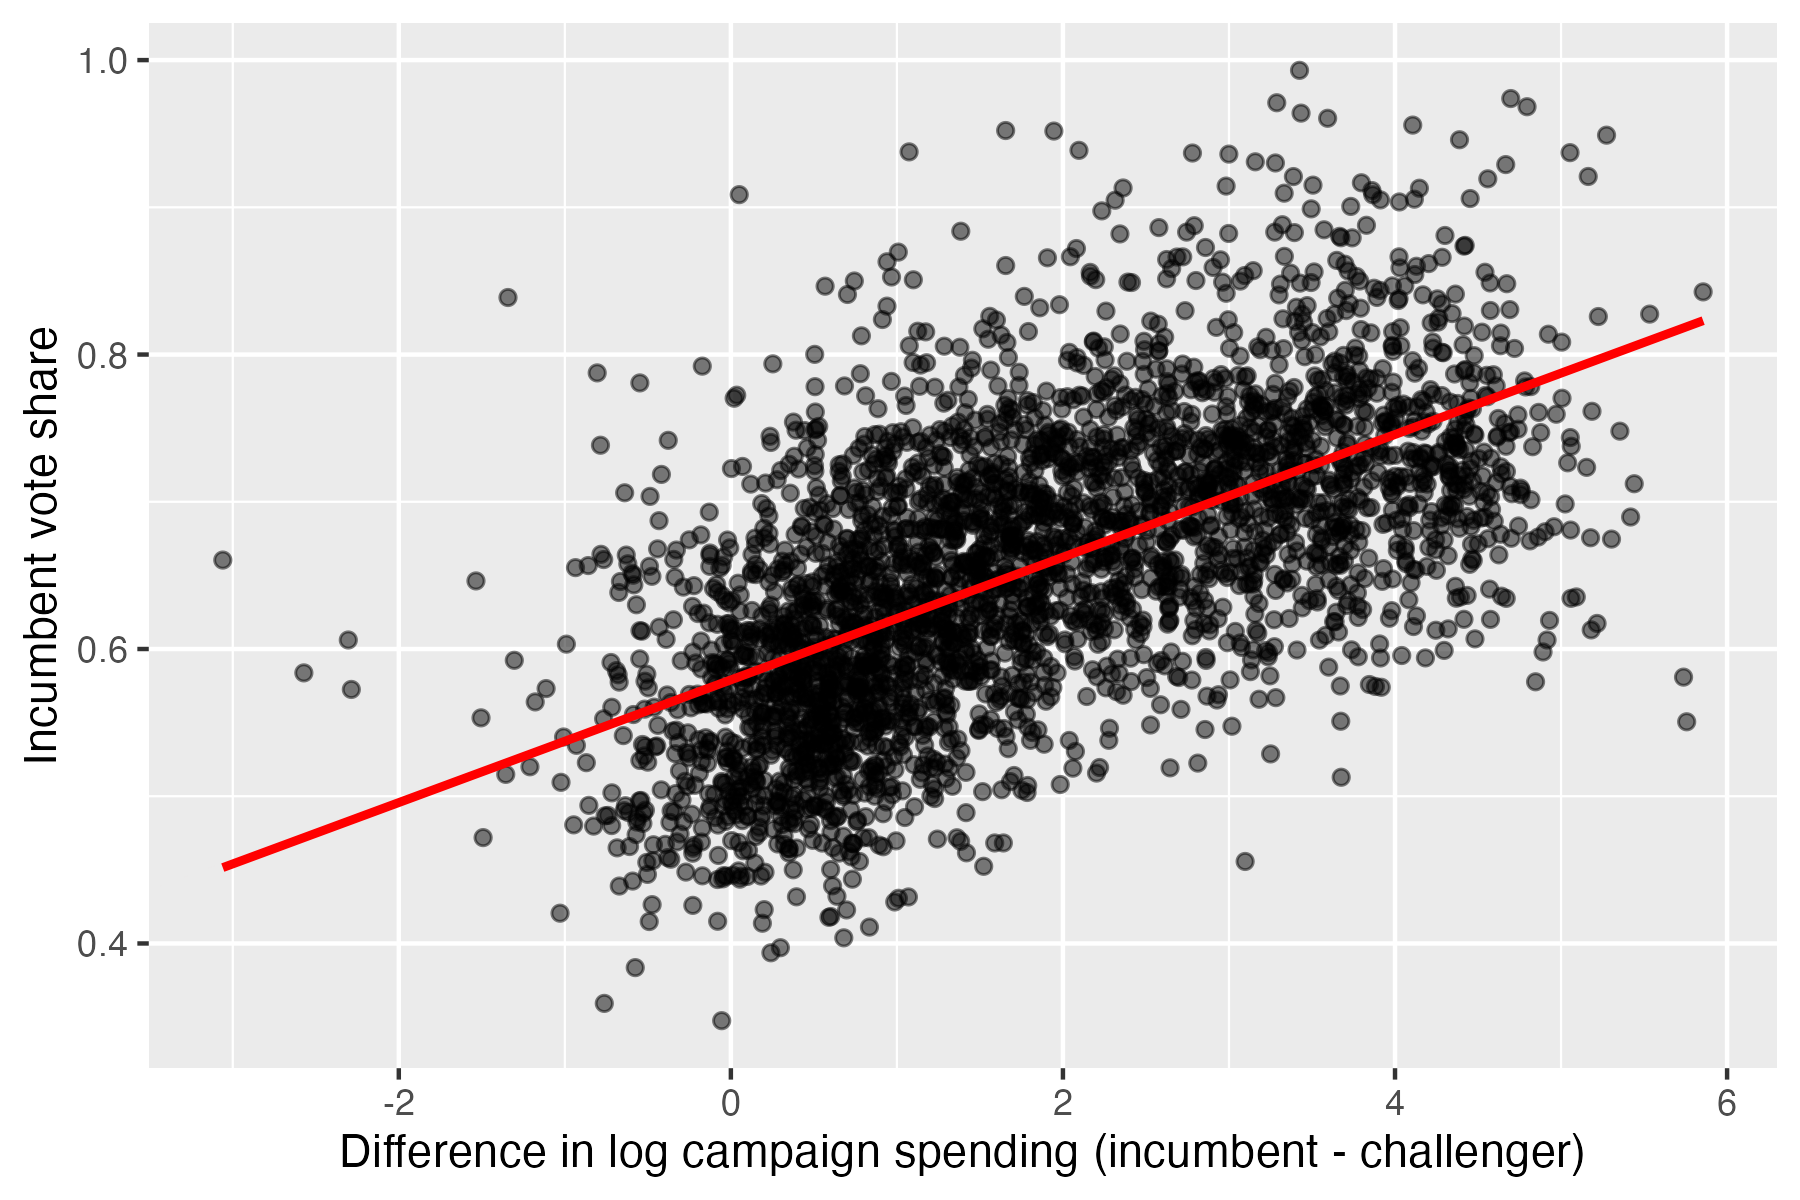
\includegraphics[width=0.8\textwidth]{q1_scatterplot.png}
  \end{center}

  \item Save the residuals of the model in a separate object.

\begin{lstlisting}[language=R]
res1 <- residuals(reg_model)
\end{lstlisting}

  \item Write the prediction equation.

  \[
    \widehat{\texttt{voteshare}} = 0.579 + 0.0417 \times \texttt{difflog}
  \]

  When the incumbent and challenger spend the same amount ($\texttt{difflog} = 0$), the predicted incumbent vote share is about 57.9\%. Each one-unit increase in \texttt{difflog} is associated with an increase of about 0.042 in vote share (roughly 4.2 percentage points). The model explains about 37\% of the variation in vote share ($R^2 = 0.367$).

\end{enumerate}
	
\newpage

\section*{Question 2}
\vspace{.25cm}
\noindent We are interested in knowing how the difference between incumbent and challenger's spending and the vote share of the presidential candidate of the incumbent's party are related.
\begin{enumerate}

  \item Run a regression where the outcome variable is \texttt{presvote} and the explanatory variable is \texttt{difflog}.

\begin{lstlisting}[language=R]
# correlation coefficient
coefficient2 <- cor.test(inc.sub$presvote, inc.sub$difflog)
coefficient2$estimate   # 0.2965653

# simple linear regression
reg_model2 <- lm(presvote ~ difflog, data = inc.sub)
summary(reg_model2)
\end{lstlisting}

  The correlation of 0.297 indicates a positive but weak-to-moderate linear relationship.

  \begin{center}
  \begin{tabular}{lcccc}
    \hline
    & Estimate & Std. Error & $t$ value & $\Pr(>|t|)$ \\
    \hline
    Intercept & 0.5076 & 0.0032 & 160.60 & $<2\times10^{-16}$ \\
    \texttt{difflog} & 0.0238 & 0.0014 & 17.54 & $<2\times10^{-16}$ \\
    \hline
  \end{tabular}
  \end{center}
  \noindent $R^2 = 0.088$, residual standard error $= 0.1104$ on 3191 degrees of freedom.

  \item Make a scatterplot of the two variables and add the regression line.

\begin{lstlisting}[language=R]
plotq2b <- inc.sub %>%
  ggplot(aes(x = difflog, y = presvote)) +
  geom_point(alpha = 0.5) +
  geom_smooth(method = "lm", se = FALSE, color = "blue") +
  labs(x = "Difference in log campaign spending (incumbent - challenger)",
       y = "Presidential candidate vote share (incumbent's party)")
plotq2b
ggsave("q2_scatterplot.png", plotq2b, width = 6, height = 4)
\end{lstlisting}

  \begin{center}
    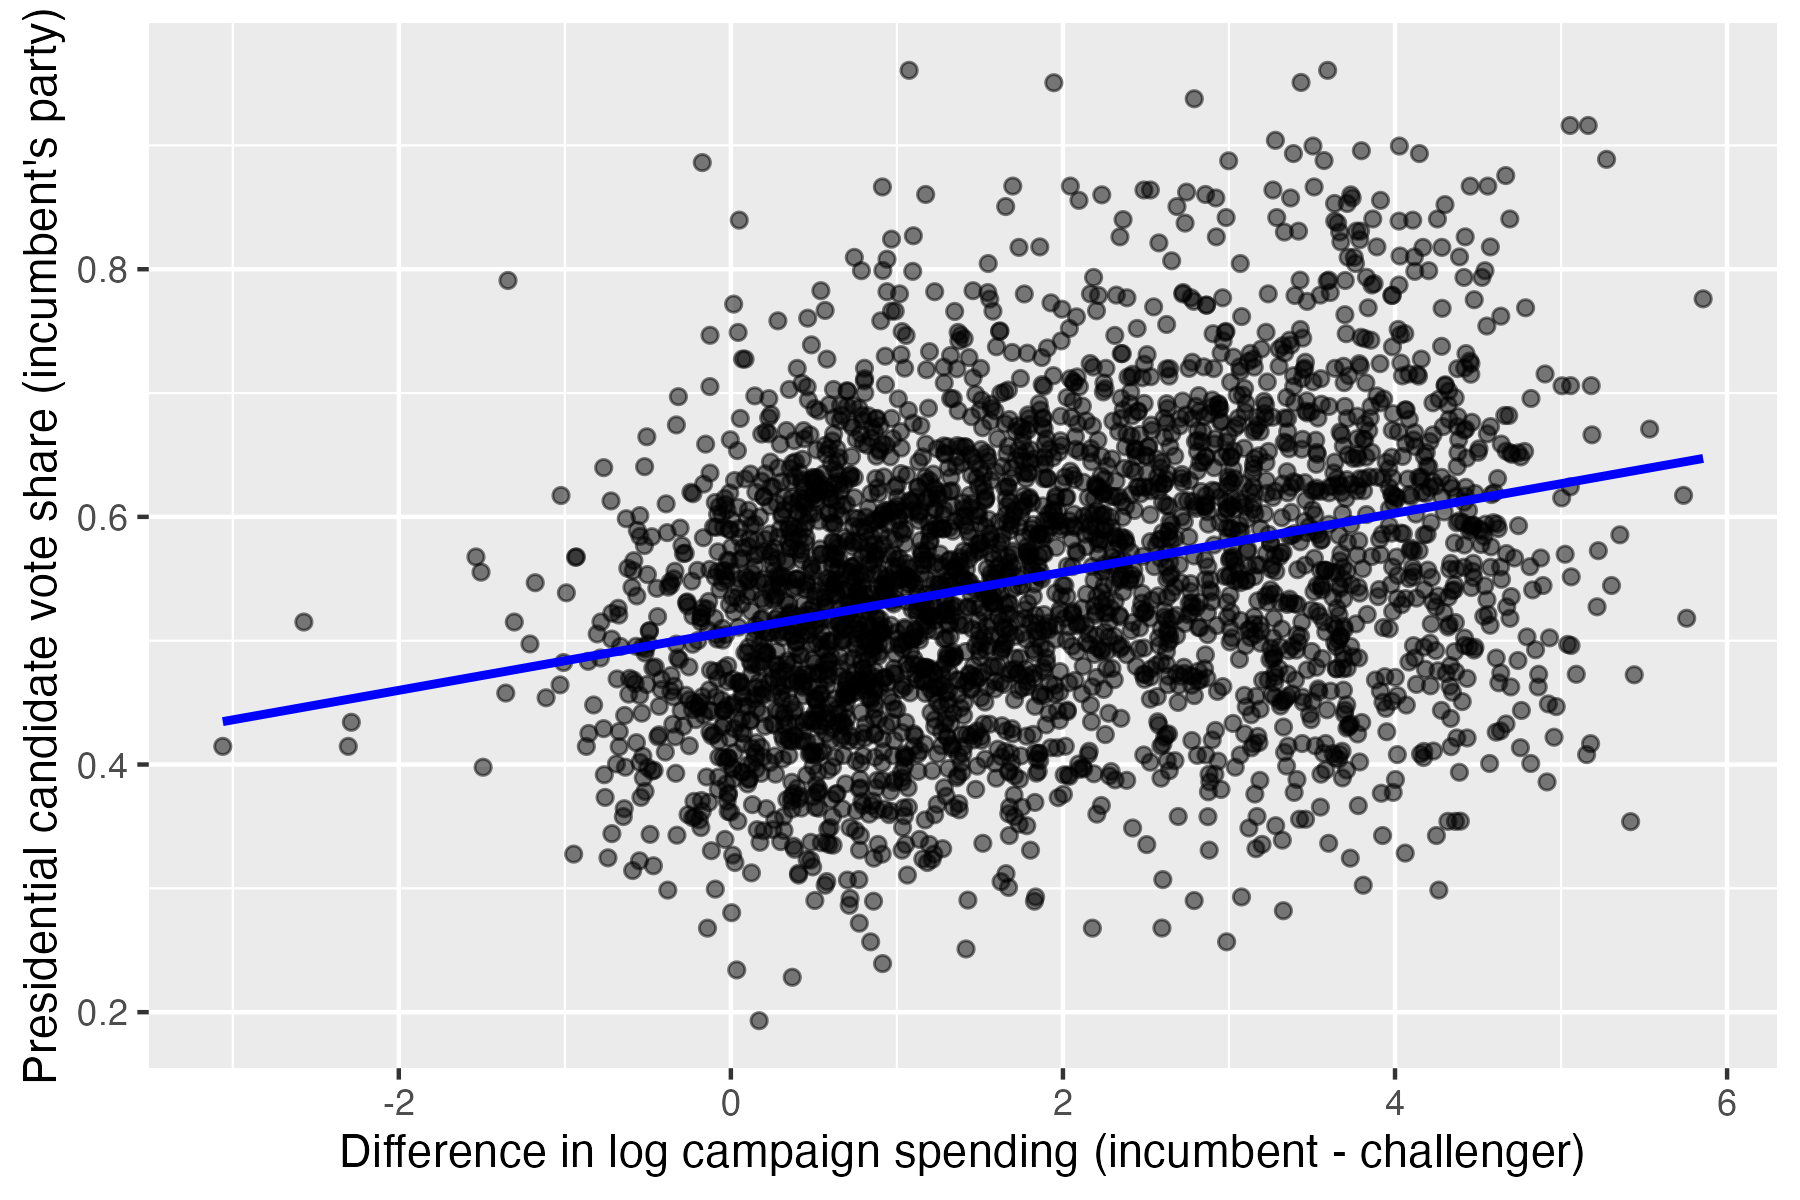
\includegraphics[width=0.8\textwidth]{q2_scatterplot.png}
  \end{center}

  \item Save the residuals of the model in a separate object.

\begin{lstlisting}[language=R]
res2 <- residuals(reg_model2)
\end{lstlisting}

  \item Write the prediction equation.

  \[
    \widehat{\texttt{presvote}} = 0.5076 + 0.0238 \times \texttt{difflog}
  \]

  When the incumbent and challenger spend the same amount ($\texttt{difflog} = 0$), the predicted vote share of the incumbent party's presidential candidate is about 50.8\%. Each one-unit increase in \texttt{difflog} is associated with an increase of about 0.024 (roughly 2.4 percentage points) in that vote share. The model explains only about 9\% of the variation in \texttt{presvote} ($R^2 = 0.088$), considerably less than the Q1 model, which explained about 37\% of the variation in \texttt{voteshare}. This is an association rather than a causal effect: a House incumbent's spending is unlikely to directly move presidential vote share, but districts that favor the incumbent's party probably produce a spending advantage and a higher presidential vote.

\end{enumerate}
	
	\newpage	
\section*{Question 3}
\vspace{.25cm}
\noindent We are interested in knowing how the vote share of the presidential candidate of the incumbent's party is associated with the incumbent's electoral success.
\begin{enumerate}

  \item Run a regression where the outcome variable is \texttt{voteshare} and the explanatory variable is \texttt{presvote}.

\begin{lstlisting}[language=R]
reg_model3 <- lm(voteshare ~ presvote, data = inc.sub)
summary(reg_model3)
\end{lstlisting}

  \begin{center}
  \begin{tabular}{lcccc}
    \hline
    & Estimate & Std. Error & $t$ value & $\Pr(>|t|)$ \\
    \hline
    Intercept & 0.4413 & 0.0076 & 58.08 & $<2\times10^{-16}$ \\
    \texttt{presvote} & 0.3880 & 0.0135 & 28.76 & $<2\times10^{-16}$ \\
    \hline
  \end{tabular}
  \end{center}
  \noindent $R^2 = 0.206$, residual standard error $= 0.0882$ on 3191 degrees of freedom.

  \item Make a scatterplot of the two variables and add the regression line.

\begin{lstlisting}[language=R]
plotq3b <- inc.sub %>%
  ggplot(aes(x = presvote, y = voteshare)) +
  geom_point(alpha = 0.5) +
  geom_smooth(method = "lm", se = FALSE, color = "yellow") +
  labs(x = "Presidential candidate vote share (incumbent's party)",
       y = "Incumbent vote share")
plotq3b
ggsave("q3_scatterplot.png", plotq3b, width = 6, height = 4)
\end{lstlisting}

  \begin{center}
    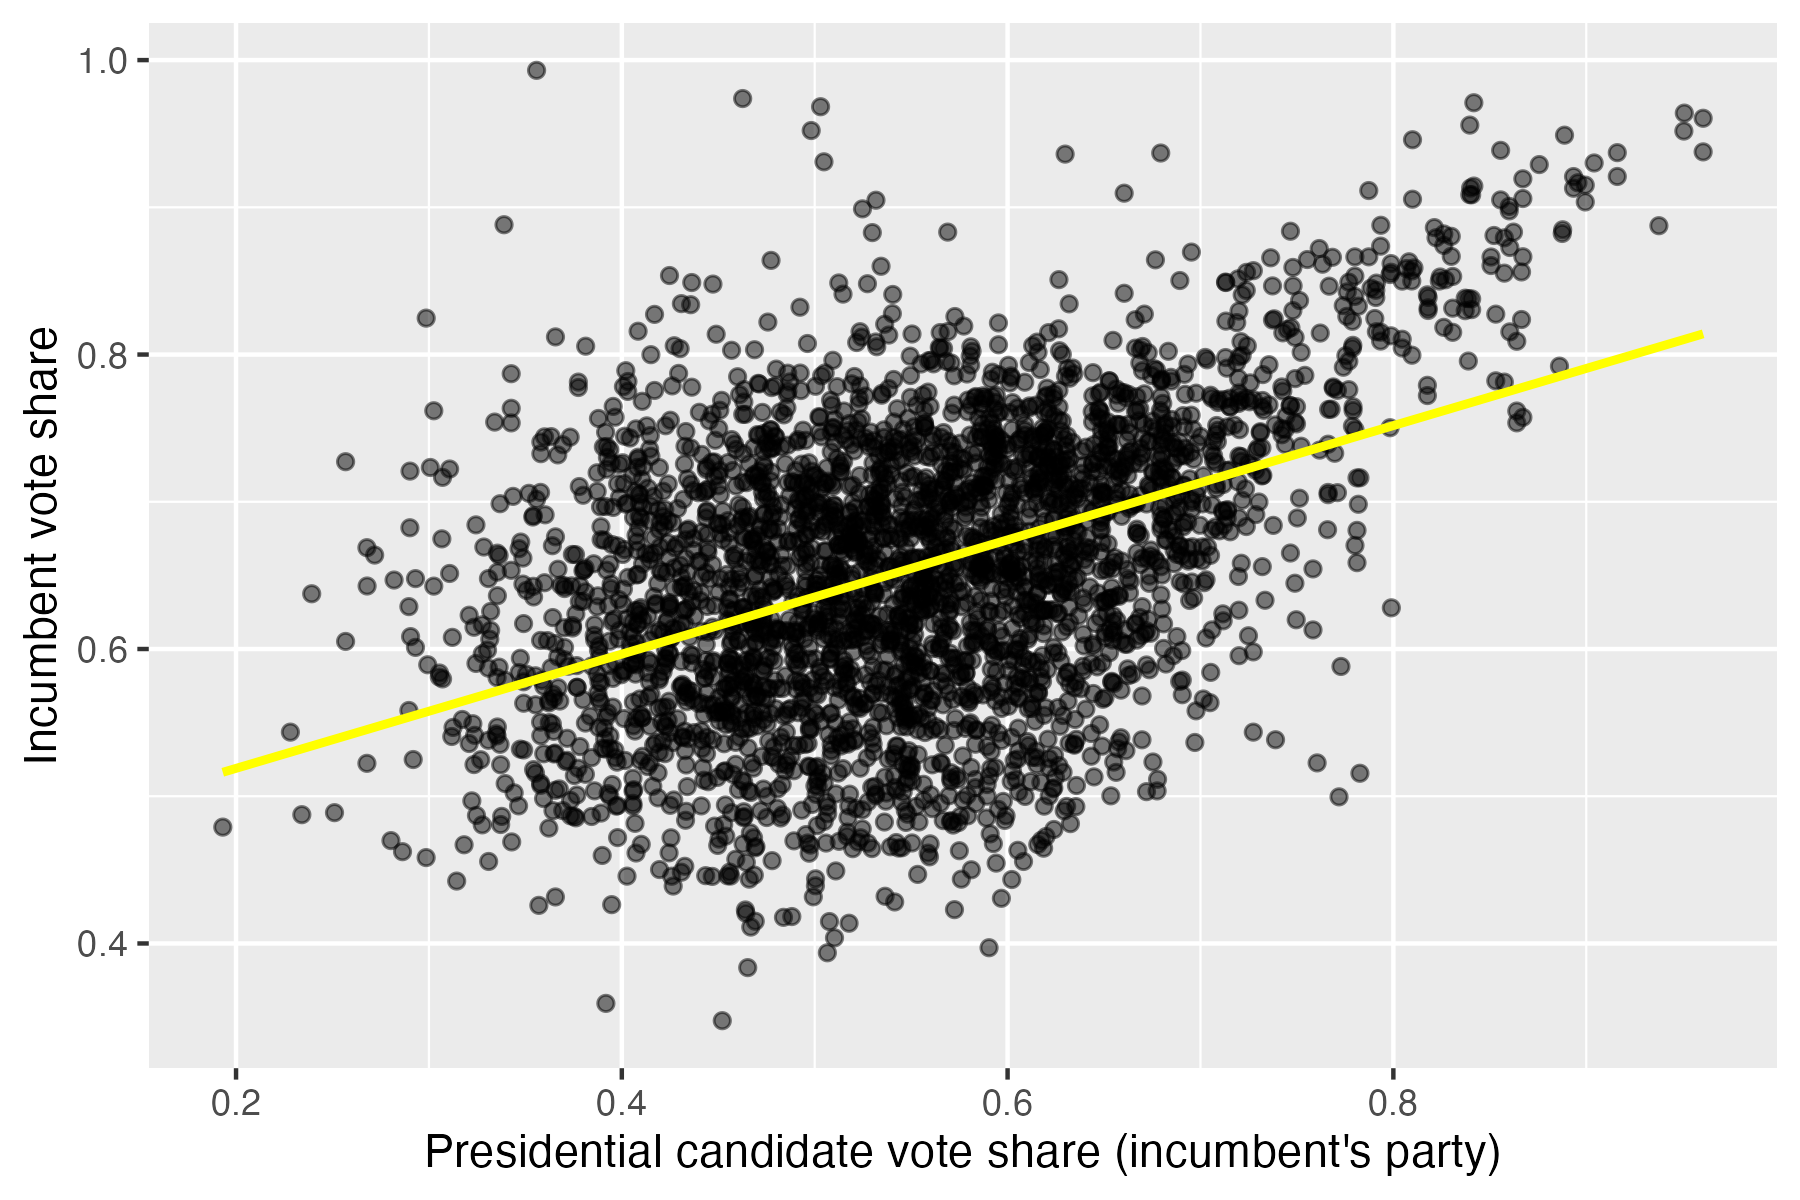
\includegraphics[width=0.8\textwidth]{q3_scatterplot.png}
  \end{center}

  \item Write the prediction equation.

  \[
    \widehat{\texttt{voteshare}} = 0.4413 + 0.3880 \times \texttt{presvote}
  \]

  Each one-unit increase in \texttt{presvote} is associated with an increase of about 0.388 in the incumbent's vote share (a 0.1 increase in \texttt{presvote} goes with about a 0.039 increase in \texttt{voteshare}). The model explains about 21\% of the variation in \texttt{voteshare}. This is an association, not a causal effect.

\end{enumerate}

\section*{Question 4}
\vspace{.25cm}
\noindent The residuals from part (a) tell us how much of the variation in \texttt{voteshare} is not explained by the difference in spending between incumbent and challenger. The residuals in part (b) tell us how much of the variation in \texttt{presvote} is not explained by the difference in spending between incumbent and challenger in the district.
\begin{enumerate}

  \item Run a regression where the outcome variable is the residuals from Question 1 and the explanatory variable is the residuals from Question 2.

\begin{lstlisting}[language=R]
reg_model4 <- lm(res ~ res2)
summary(reg_model4)
\end{lstlisting}

  \begin{center}
  \begin{tabular}{lcccc}
    \hline
    & Estimate & Std. Error & $t$ value & $\Pr(>|t|)$ \\
    \hline
    Intercept & $\approx 0$ & 0.0013 & 0.00 & 1 \\
    \texttt{res2} & 0.2569 & 0.0118 & 21.84 & $<2\times10^{-16}$ \\
    \hline
  \end{tabular}
  \end{center}
  \noindent $R^2 = 0.130$, residual standard error $= 0.0734$ on 3191 degrees of freedom.

  \item Make a scatterplot of the two residuals and add the regression line.

\begin{lstlisting}[language=R]
plotq4b <- ggplot(data.frame(res1 = res1, res2 = res2), aes(x = res2, y = res1)) +
  geom_point(alpha = 0.5) +
  geom_smooth(method = "lm", se = FALSE, color = "green") +
  labs(x = "Residuals of presvote ~ difflog (Q2)",
       y = "Residuals of voteshare ~ difflog (Q1)")
plotq4b
ggsave("q4_scatterplot.png", plotq4b, width = 6, height = 4)
\end{lstlisting}

  \begin{center}
    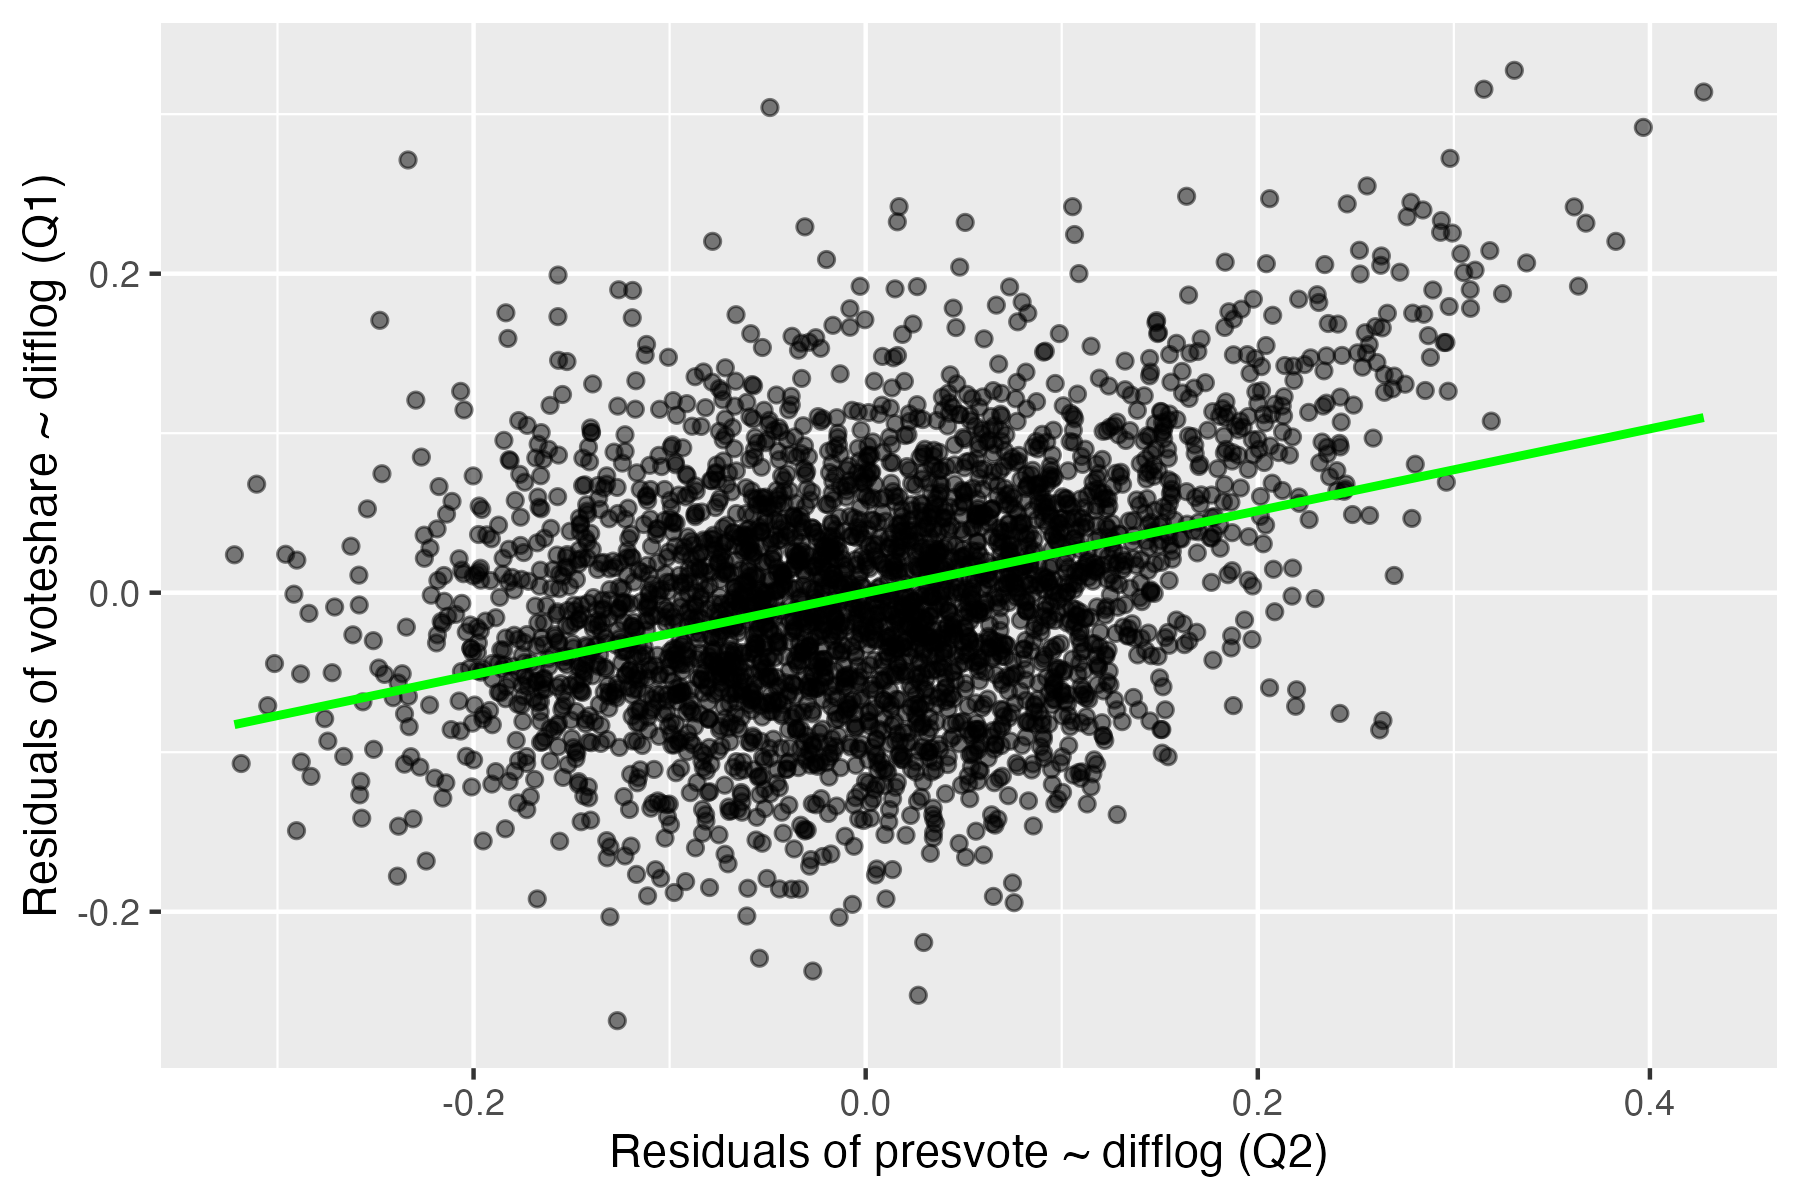
\includegraphics[width=0.8\textwidth]{q4_scatterplot.png}
  \end{center}

  \item Write the prediction equation.

  \[
    \widehat{res} = 0 + 0.2569 \times res2
  \]

  The intercept is zero (up to rounding error) because residuals from a regression with an intercept always have a mean of zero, so the fitted line passes through the origin.
  The positive slope means districts where the presidential candidate overperformed relative to spending also tend to see the incumbent overperform.
\end{enumerate}
	
	\newpage	

\section*{Question 5}
\vspace{.25cm}
\noindent What if the incumbent's vote share is affected by both the president's popularity and the difference in spending between incumbent and challenger?
\begin{enumerate}

  \item Run a regression where the outcome variable is the incumbent's \texttt{voteshare} and the explanatory variables are \texttt{difflog} and \texttt{presvote}.

\begin{lstlisting}[language=R]
reg_model5 <- lm(voteshare ~ difflog + presvote, data = inc.sub)
summary(reg_model5)
\end{lstlisting}

  \begin{center}
  \begin{tabular}{lcccc}
    \hline
    & Estimate & Std. Error & $t$ value & $\Pr(>|t|)$ \\
    \hline
    Intercept & 0.4486 & 0.0063 & 70.88 & $<2\times10^{-16}$ \\
    \texttt{difflog} & 0.0355 & 0.0009 & 37.59 & $<2\times10^{-16}$ \\
    \texttt{presvote} & 0.2569 & 0.0118 & 21.84 & $<2\times10^{-16}$ \\
    \hline
  \end{tabular}
  \end{center}
  \noindent $R^2 = 0.450$, residual standard error $= 0.0734$ on 3190 degrees of freedom.

  \item Write the prediction equation.

  \[
    \widehat{\texttt{voteshare}} = 0.4486 + 0.0355 \times \texttt{difflog} + 0.2569 \times \texttt{presvote}
  \]

  \item What is it in this output that is identical to the output in Question 4? Why do you think this is the case?

  	The slope on res2 is the same as the presvote coefficient in Q5- the plot shows the relationship between voteshare and presvote after difflog is removed from both. The coefficient on \texttt{presvote} in Q5 (0.2569) is identical to the slope on the residuals of Q2 in Q4 (0.2569). In Q4, the residuals from Q1 are the part of \texttt{voteshare} not explained by \texttt{difflog}, and the residuals from Q2 are the part of \texttt{presvote} not explained by \texttt{difflog}. Regressing one on the other therefore isolates the relationship between \texttt{presvote} and \texttt{voteshare} after removing the influence of \texttt{difflog} from both. This is exactly what a multiple regression coefficient represents: the association between \texttt{presvote} and \texttt{voteshare} holding \texttt{difflog} constant, or without  \texttt{difflog} influence. 

\end{enumerate}




\end{document}
